\documentclass[conference]{IEEEtran}

% ── Paquetes ──────────────────────────────────────────────────────
\usepackage[utf8]{inputenc}
\usepackage[spanish,es-nodecimaldot]{babel}
\usepackage{graphicx}
\usepackage{amsmath,amssymb}
\usepackage{booktabs}
\usepackage{tabularx}
\usepackage[hidelinks]{hyperref}
\usepackage{float}
\usepackage{xcolor}
\usepackage{colortbl}
\usepackage{cite}
\usepackage{url}
\usepackage{multirow}
\usepackage{makecell}

% ── Colores para celdas de tabla ─────────────────────────────────
\definecolor{cellgood}{RGB}{212,237,218}
\definecolor{cellmid}{RGB}{255,243,205}
\definecolor{cellbad}{RGB}{248,215,218}

% ── Metadatos ────────────────────────────────────────────────────
\title{Segmentación clásica de gliomas en BraTS 2024 (GLI) y
registro rígido por información mutua: un estudio de las
limitaciones de los métodos sin aprendizaje profundo}

\author{\IEEEauthorblockN{Abel Albuez, Victoria Acero y Santiago Gil}
\IEEEauthorblockA{Maestría en Ingeniería de Sistemas y Computación\\
Pontificia Universidad Javeriana, Bogotá D.C., Colombia\\
Procesamiento de Imágenes Médicas \quad 2026\\
Repositorio: \url{https://github.com/AbelAlbuez/medical-image-processing}}}

\begin{document}

\maketitle

% ── Abstract ─────────────────────────────────────────────────────
\begin{abstract}
Se presenta un proyecto de procesamiento de imágenes médicas
sobre el dataset \textit{BraTS 2024 Adult Glioma} (GLI),
estructurado en tres bloques: (i) un análisis exploratorio (EDA)
de 25 casos multimodales (T1n, T1c, T2w, T2-FLAIR); (ii) un
pipeline de segmentación automática del tumor cerebral
\emph{completo} (\texttt{seg > 0}) en la modalidad FLAIR mediante
métodos clásicos basados en intensidad ---Otsu multinivel,
modelos de mezcla Gaussiana (GMM), crecimiento de regiones
sembrado en el centroide del \emph{ground truth} y watershed por
marcadores--- sin recurrir a aprendizaje profundo; y (iii) una
demostración cuantitativa de registro rígido por información mutua
de Mattes con transformación Euler3D y esquema multi-resolución,
sobre tres casos representativos. El hallazgo central del bloque
de segmentación es que los métodos puramente basados en intensidad
son \textbf{insuficientes} para el tumor completo en casos
post-tratamiento (Dice medio $0{,}33$ con Otsu, el mejor método;
$0{,}18$ con crecimiento de regiones), principalmente porque la
cavidad de resección es hipointensa en FLAIR y rompe la hipótesis
de un único modo brillante. El registro, en cambio, recupera la
perturbación rígida impuesta con un \emph{Target Registration
Error} (TRE) residual sub-vóxel (media $0{,}004$~mm), confirmando
la robustez del motor Mattes\,MI\,+\,Euler3D incluso cuando las
modalidades del dataset ya están coregistradas de fábrica.
\end{abstract}

\begin{IEEEkeywords}
BraTS 2024, gliomas, segmentación clásica, Otsu, GMM,
crecimiento de regiones, watershed, registro rígido,
información mutua, ITK, SimpleITK.
\end{IEEEkeywords}

% =====================================================================
\section{Introducción y objetivos}
\label{sec:intro}
% =====================================================================
Los gliomas adultos son los tumores cerebrales primarios más
frecuentes y presentan una alta heterogeneidad morfológica e
intensitaria que dificulta su delineación automática en
resonancia magnética (RM). La iniciativa BraTS (\textit{Brain
Tumor Segmentation Challenge}) provee anualmente un dataset
multimodal con segmentaciones expertas que se ha convertido en
el estándar de facto para evaluar algoritmos de segmentación de
gliomas~\cite{baid2021brats}. La edición 2024 (track GLI) amplía
la cohorte y reorganiza las etiquetas para distinguir entre
\emph{Necrotic Tumor Core} (NETC), \emph{Surrounding Non-enhancing
FLAIR Hyperintensity} (SNFH), \emph{Enhancing Tumor} (ET) y
\emph{Resection Cavity} (RC).

El presente proyecto se enmarca en el curso de Procesamiento de
Imágenes Médicas de la Maestría en Ingeniería de Sistemas y
Computación de la Pontificia Universidad Javeriana, cuyo requisito
explícito es resolver tareas de análisis de imagen \textbf{sin
recurrir a aprendizaje profundo}. Bajo esa restricción, los
objetivos son:
\begin{enumerate}
  \item Caracterizar mediante un EDA cuantitativo el dataset
        BraTS 2024 GLI y derivar parámetros operativos (modalidad
        fija para registro, métrica recomendada, semillas).
  \item Implementar un pipeline reproducible de \textbf{segmentación
        automática del tumor completo} (\texttt{seg > 0}) sobre la
        modalidad T2-FLAIR usando cuatro familias clásicas (Otsu,
        GMM, crecimiento de regiones, watershed) y cuantificar
        sus límites contra \emph{ground truth}.
  \item Demostrar cuantitativamente, sobre tres casos, un motor de
        \textbf{registro rígido por información mutua} (Mattes\,MI
        + Euler3D multi-resolución) recuperando una perturbación
        conocida.
\end{enumerate}
La hipótesis de trabajo es que, aun con una cuidadosa cadena de
preprocesamiento (Wiener + N4 + normalización por percentiles),
los métodos clásicos basados solamente en intensidad serán
insuficientes para casos con cavidad de resección, justificando
empíricamente la necesidad de información de forma, atlas o
aprendizaje en pipelines clínicos modernos.

% =====================================================================
\section{Materiales y dataset}
\label{sec:dataset}
% =====================================================================
Se trabajó sobre una muestra de \textbf{25 casos} del subconjunto
público BraTS 2024 GLI. Cada caso contiene cuatro volúmenes
multimodales 3D ---T1 nativo (T1n), T1 con contraste (T1c), T2
ponderado (T2w) y T2 FLAIR (T2f)--- y una segmentación experta
(\texttt{seg}) con las etiquetas NETC, SNFH, ET y RC. Como
muestra la Tabla~\ref{tab:geometria}, los 25 volúmenes comparten
geometría exactamente: forma $182\times 218\times 182$, espaciado
isotrópico de $1\,$mm y orientación LAS, lo que descarta la
necesidad de remuestreo o reorientación previas.

\begin{table}[H]
\centering
\caption{Geometría de los 25 casos analizados (homogénea en
todo el subset).}
\label{tab:geometria}
\small
\begin{tabular}{lc}
\toprule
Propiedad & Valor \\
\midrule
Forma del volumen (vóxeles) & $182\times 218\times 182$ \\
Espaciado (mm)             & $1{,}00 \times 1{,}00 \times 1{,}00$ \\
Orientación                 & LAS \\
Casos isotrópicos a 1\,mm  & 100\% \\
\bottomrule
\end{tabular}
\end{table}

\subsection{Distribución de intensidades por modalidad}
La Figura~\ref{fig:eda_intensidad} resume la distribución de
intensidades por modalidad sobre los 25 casos. Las cuatro
modalidades difieren tanto en rango dinámico como en forma del
histograma, motivando la normalización por percentiles que se
describe en la Sección~\ref{sec:preproc}.

\begin{figure}[H]
\centering
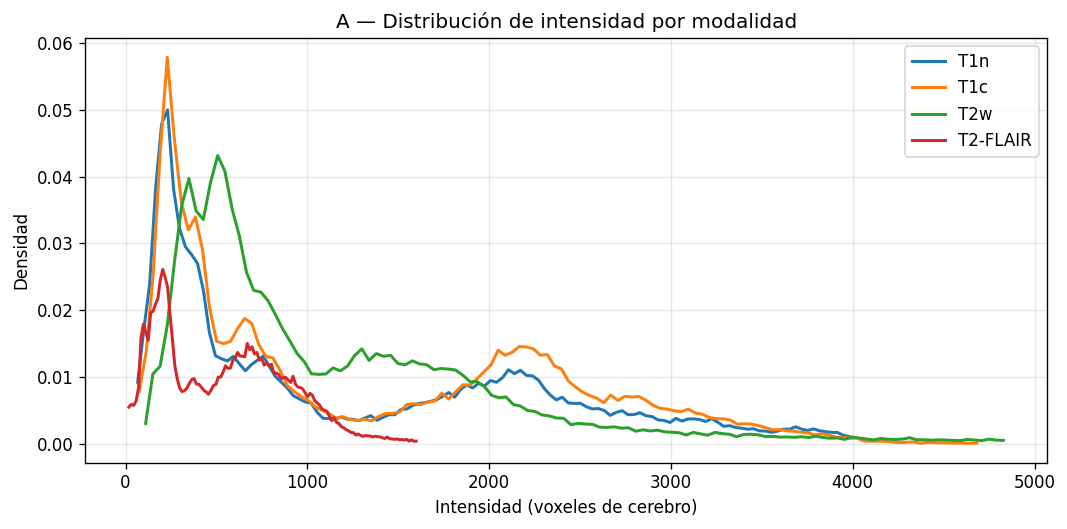
\includegraphics[width=\columnwidth]{figuras/eda_intensidad_modalidad.png}
\caption{Distribuciones de intensidad por modalidad sobre los 25
casos (T1n, T1c, T2w, T2-FLAIR).}
\label{fig:eda_intensidad}
\end{figure}

\subsection{Separabilidad sub-región vs.\ tejido sano}
Para anticipar el desempeño esperado de una segmentación por
umbral, se calcularon dos métricas de separabilidad entre cada
sub-región y el tejido sano: el \emph{Fisher Discriminant Ratio}
(FDR; mayor = más separable) y la distancia de Bhattacharyya
(mayor = más separable). Los valores se reportan en la
Tabla~\ref{tab:separabilidad}.

\begin{table}[H]
\centering
\caption{Separabilidad de cada sub-región respecto a tejido
sano, por modalidad. \emph{FDR}: Fisher Discriminant Ratio
(\;$\uparrow$ mejor\;). \emph{Bhatt.}: distancia de
Bhattacharyya (\;$\uparrow$ mejor\;).}
\label{tab:separabilidad}
\small
\begin{tabular}{llcccc}
\toprule
Métrica & Sub-región & T1n & T1c & T2w & T2-FLAIR \\
\midrule
\multirow{4}{*}{FDR}
 & NETC & 0.611 & 0.672 & 0.551 & 0.550 \\
 & SNFH & 0.851 & 0.858 & 0.740 & 0.604 \\
 & ET   & 0.663 & 0.731 & 0.710 & 0.670 \\
 & RC   & 0.639 & 0.638 & 0.564 & 0.659 \\
\midrule
\multirow{4}{*}{Bhatt.}
 & NETC & 0.145 & 0.079 & 0.204 & 0.211 \\
 & SNFH & 0.026 & 0.018 & 0.057 & \textbf{0.163} \\
 & ET   & 0.089 & 0.070 & 0.069 & 0.089 \\
 & RC   & 0.134 & 0.134 & 0.188 & 0.082 \\
\bottomrule
\end{tabular}
\end{table}

La SNFH (edema/infiltración no-realzante, principal componente
del \emph{tumor completo}) es claramente más separable en T2-FLAIR
($\mathrm{Bhatt.}=0{,}163$ frente a $\leq 0{,}06$ en las otras
modalidades). Este resultado justifica empíricamente la elección
de FLAIR como modalidad de trabajo para la segmentación del
objetivo \texttt{seg > 0}.

\begin{figure}[H]
\centering
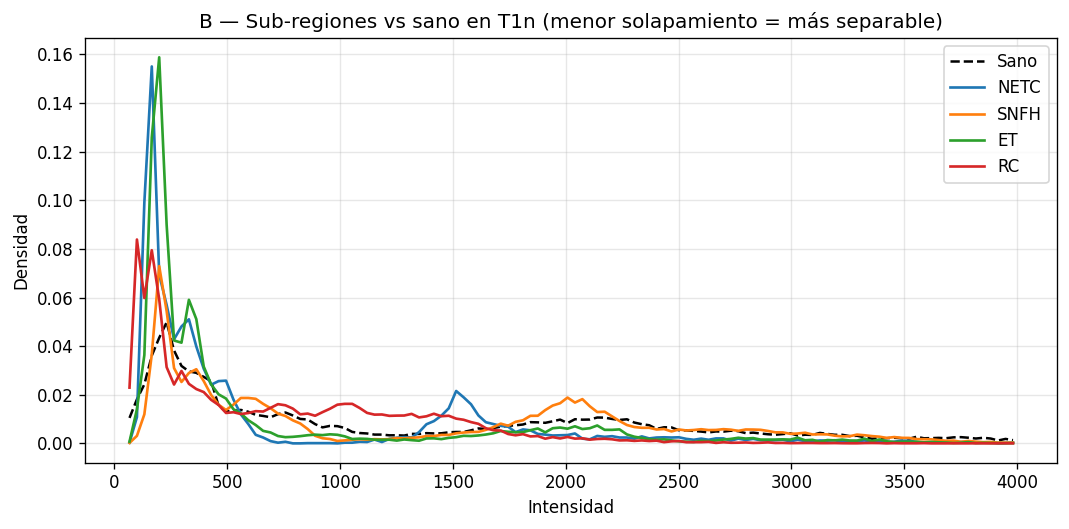
\includegraphics[width=\columnwidth]{figuras/eda_separabilidad.png}
\caption{Separabilidad sub-región vs.\ tejido sano: heatmaps
de FDR y Bhattacharyya por modalidad y sub-región.}
\label{fig:eda_sep}
\end{figure}

\subsection{Umbrales Otsu y grado de bimodalidad}
Se estimaron umbrales Otsu multinivel (dos cortes) sobre cada
modalidad y se cuantificó el grado de bimodalidad del histograma
(razón inter/intra-clase). Como referencia global, la
Tabla~\ref{tab:otsu} reporta los valores medianos.

\begin{table}[H]
\centering
\caption{Umbrales Otsu multinivel medianos y bimodalidad por
modalidad (sobre 25 casos).}
\label{tab:otsu}
\small
\begin{tabular}{lccc}
\toprule
Modalidad & Otsu bajo & Otsu alto & Bimodalidad \\
\midrule
T1c       & 759.17 & 1710.55 & 0.229 \\
T1n       & 505.17 &  822.55 & 0.533 \\
T2-FLAIR  & 393.97 &  698.63 & 0.369 \\
T2w       & 791.70 & 1332.09 & \textbf{0.587} \\
\bottomrule
\end{tabular}
\end{table}

\begin{figure}[H]
\centering
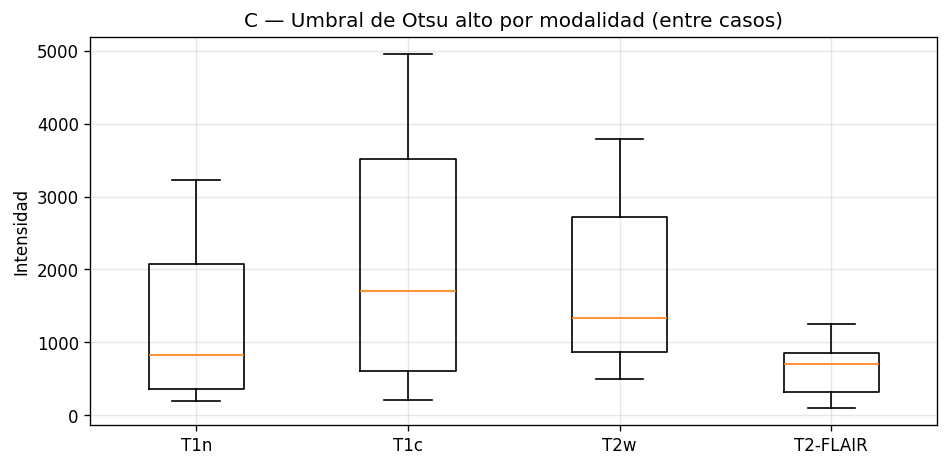
\includegraphics[width=\columnwidth]{figuras/eda_otsu_bimodalidad.png}
\caption{Umbrales Otsu (líneas verticales) sobre el histograma
agregado y grado de bimodalidad por modalidad.}
\label{fig:eda_otsu}
\end{figure}

\subsection{Variabilidad inter-caso y casos demostrativos}
Existe una alta varianza inter-caso del volumen tumoral total
(de $\sim$\,$4{,}5\,$k vóxeles en el caso más pequeño hasta
$\sim$\,$195\,$k en el más grande), así como del p99 de intensidad.
La Figura~\ref{fig:eda_var} ilustra esa dispersión. Para los
bloques de segmentación y registro se eligieron cinco casos
representativos cubriendo distintas situaciones clínicas, listados
en la Tabla~\ref{tab:demo}.

\begin{figure}[H]
\centering
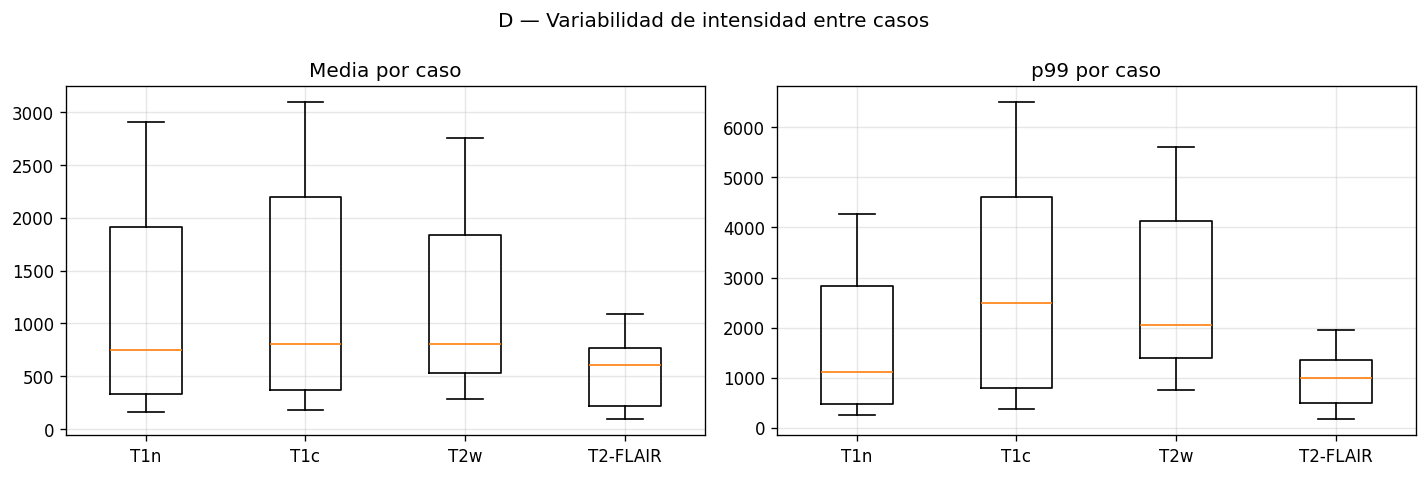
\includegraphics[width=\columnwidth]{figuras/eda_variabilidad_casos.png}
\caption{Variabilidad inter-caso de las medias y p99 de
intensidad por modalidad.}
\label{fig:eda_var}
\end{figure}

\begin{table}[H]
\centering
\caption{Cinco casos demostrativos seleccionados para los
experimentos. Volúmenes en vóxeles (ground truth).}
\label{tab:demo}
\small
\setlength{\tabcolsep}{4pt}
\begin{tabular}{llrrrrr}
\toprule
Caso & Motivo & Total & NETC & SNFH & ET & RC \\
\midrule
02827-100 & Típico (mediana)        & 57050 & 0    & 13208  & 0    & 43842 \\
02119-101 & Tumor grande ($\sim$p95)& 195115& 2701 & 174405 & 2409 & 15600 \\
02923-101 & Tumor pequeño ($\sim$p5)& 10036 & 0    & 4798   & 0    & 5238 \\
02514-102 & Post-resección (RC$>0$)  & 156341& 0    & 62326  & 5185 & 88830 \\
02859-100 & Sólo edema (sin ET)     & 64735 & 0    & 62422  & 0    & 2313 \\
\bottomrule
\end{tabular}
\end{table}

Nótese que en cuatro de los cinco casos la sub-región
\emph{Resection Cavity} (RC) es significativa, y en tres de ellos
es la sub-región dominante. Esto será determinante para entender
las limitaciones reportadas en la Sección~\ref{sec:disc}.

\subsection{Semilla automática para crecimiento de regiones}
Como insumo del método de crecimiento de regiones se identificó,
por caso, un punto candidato a semilla preferentemente dentro de
ET (o, en su defecto, dentro del tumor completo) con su intensidad
T1c asociada. La Figura~\ref{fig:eda_seed} muestra el
solapamiento de las intensidades de semilla con la distribución
de tejido sano, anticipando que la semilla por sí sola no es
discriminante.

\begin{figure}[H]
\centering
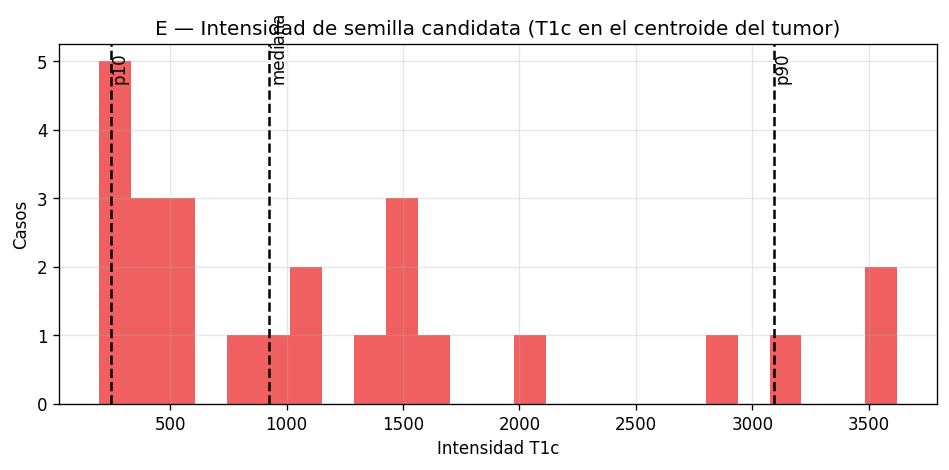
\includegraphics[width=\columnwidth]{figuras/eda_semilla_t1c.png}
\caption{Intensidades T1c en el voxel semilla (por caso) frente
a la distribución global de T1c en tejido sano.}
\label{fig:eda_seed}
\end{figure}

\subsection{Parámetros derivados para el bloque de registro}
A partir del EDA (archivo \texttt{parametros\_registro.json}) se
fijaron los parámetros operativos del registro: modalidad fija
recomendada \textbf{T1n}, métrica \textbf{Información Mutua de
Mattes} (apropiada para escenarios multimodales), transformación
\textbf{rígida Euler3D} y un \textbf{100\%} de casos
isotrópicos a $1\,$mm. Crucialmente, el EDA verifica que las
cuatro modalidades por caso ya están coregistradas, por lo que
el registro intra-sujeto es \emph{redundante} y se plantea como
un ejercicio \textbf{demostrativo} (perturbación rígida conocida
$\to$ recuperación).

% =====================================================================
\section{Preprocesamiento}
\label{sec:preproc}
% =====================================================================
Antes de toda segmentación se aplica un pipeline de limpieza de
intensidades común a todos los métodos, encadenado en el orden:

\begin{enumerate}
  \item \textbf{Filtro de Wiener} con kernel de tamaño $3$ para
        atenuar ruido gaussiano sin penalizar bordes.
  \item \textbf{Corrección de campo de sesgo N4} (Tustison
        \emph{et al.}~\cite{tustison2010n4}) con factor de
        \emph{shrink}$=4$ para eliminar el sesgo lento de
        intensidad típico de RM.
  \item \textbf{Normalización por percentiles}: recorte al
        intervalo $[p_{0{,}5}, p_{99{,}5}]$ y reescalado lineal a
        $[0,1]$ por volumen, descartando los extremos sin
        eliminar señal anatómica relevante.
\end{enumerate}

El volumen normalizado se almacena en
\texttt{limpieza/<caso>/<caso>-t2f\_limpio.npy} y constituye la
entrada única para los cuatro métodos de segmentación de la
Sección~\ref{sec:seg}. La razón de aplicar la limpieza a FLAIR
(\texttt{t2f}) es la conclusión del EDA: FLAIR es la modalidad
con mayor separabilidad para el SNFH/tumor-completo.

% =====================================================================
\section{Segmentación clásica del tumor completo}
\label{sec:seg}
% =====================================================================
Se implementaron cuatro familias clásicas de segmentación, todas
operando sobre el mismo volumen FLAIR preprocesado y con el mismo
objetivo: producir una máscara binaria del \textbf{tumor completo}
(unión de NETC, SNFH, ET y RC, es decir, \texttt{seg > 0}).

\subsection{Métodos}
\begin{description}
  \item[Otsu multinivel.] Umbralización por Otsu con dos cortes
        y selección de la clase de mayor intensidad
        (\emph{foreground} $=$ tumor candidato).
  \item[Modelos de mezcla Gaussiana (GMM).] Ajuste de una mezcla
        de tres componentes sobre los vóxeles del cerebro
        enmascarado; la clase con mayor media se toma como
        candidata a tumor.
  \item[Crecimiento de regiones (\texttt{ConnectedThreshold} de
        ITK).] Sembrado automáticamente en el \emph{centroide del
        ground truth} del tumor completo y propagado a vecinos
        dentro de una banda de intensidad calibrada en torno a
        la intensidad de semilla.
  \item[Watershed por marcadores.] Watershed morfológico sobre la
        magnitud del gradiente del volumen FLAIR, con marcadores
        derivados de mínimos regionales y de la propia máscara
        Otsu como restricción de \emph{foreground}.
\end{description}

\subsection{Métricas y configuración experimental}
La evaluación se realizó sobre los cinco casos demostrativos de
la Tabla~\ref{tab:demo}. Como verdad terreno se usó
\texttt{seg > 0} (tumor completo). Se reportan Dice, Jaccard y
sensibilidad ($TP/(TP+FN)$) por método y caso.

\subsection{Resultados agregados}
La Tabla~\ref{tab:seg_resumen} resume las métricas promediadas
sobre los cinco casos. Otsu obtiene el mejor Dice agregado pero
con un valor bajo ($0{,}325$); el crecimiento de regiones
\textbf{falla completamente} (Dice $\approx 0{,}18$, sensibilidad
$0{,}16$). La Figura~\ref{fig:seg_metricas} ilustra el ranking de
métodos.

\begin{table}[H]
\centering
\caption{Métricas promedio sobre los 5 casos demostrativos
(objetivo: tumor completo, modalidad FLAIR).}
\label{tab:seg_resumen}
\small
\begin{tabular}{lccc}
\toprule
Método        & Dice  & Jaccard & Sensibilidad \\
\midrule
Otsu          & \cellcolor{cellmid}\textbf{0.325} & \cellcolor{cellmid}\textbf{0.255} & \cellcolor{cellmid}0.583 \\
Watershed     & 0.239 & 0.196 & \cellcolor{cellmid}\textbf{0.638} \\
GMM           & 0.208 & 0.184 & 0.400 \\
Crecimiento   & \cellcolor{cellbad}0.179 & \cellcolor{cellbad}0.162 & \cellcolor{cellbad}0.163 \\
\bottomrule
\end{tabular}
\end{table}

\begin{figure}[H]
\centering
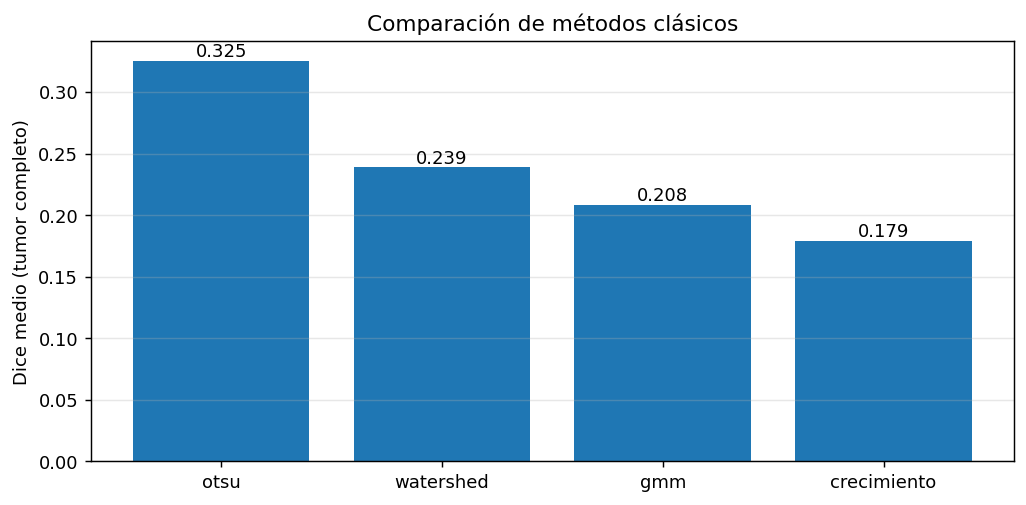
\includegraphics[width=\columnwidth]{figuras/seg_metricas.png}
\caption{Comparativa visual de métricas (Dice, Jaccard,
sensibilidad) por método clásico sobre los 5 casos.}
\label{fig:seg_metricas}
\end{figure}

\subsection{Resultados por caso}
El detalle por caso (Tabla~\ref{tab:seg_detalle}) revela un patrón
muy informativo: \emph{los cuatro métodos rinden bien únicamente
en el caso de tumor grande sin cavidad dominante} (02119-101,
Dice $\geq 0{,}89$ para Otsu, GMM y crecimiento), y todos colapsan
en presencia de cavidad de resección o ausencia total de ET.

\begin{table}[H]
\centering
\caption{Dice por caso y método (objetivo tumor completo, FLAIR).
Codificación: \emph{verde} Dice$\geq 0{,}80$; \emph{amarillo}
$0{,}50$--$0{,}80$; \emph{rojo} $<0{,}50$.}
\label{tab:seg_detalle}
\small
\setlength{\tabcolsep}{4pt}
\begin{tabular}{lcccc}
\toprule
Caso         & Otsu  & GMM   & Crecim. & Watershed \\
\midrule
02827-100 (típico, RC dom.)
 & \cellcolor{cellbad}0.027 & \cellcolor{cellbad}0.025 & \cellcolor{cellbad}0.000 & \cellcolor{cellbad}0.023 \\
02119-101 (tumor grande)
 & \cellcolor{cellgood}0.896 & \cellcolor{cellgood}0.924 & \cellcolor{cellgood}0.896 & \cellcolor{cellgood}0.905 \\
02923-101 (tumor pequeño)
 & \cellcolor{cellbad}0.014 & \cellcolor{cellbad}0.013 & \cellcolor{cellbad}0.000 & \cellcolor{cellbad}0.010 \\
02514-102 (post-resección)
 & \cellcolor{cellmid}0.508 & \cellcolor{cellbad}0.057 & \cellcolor{cellbad}0.000 & \cellcolor{cellbad}0.141 \\
02859-100 (solo edema)
 & \cellcolor{cellbad}0.182 & \cellcolor{cellbad}0.023 & \cellcolor{cellbad}0.000 & \cellcolor{cellbad}0.115 \\
\bottomrule
\end{tabular}
\end{table}

Las figuras~\ref{fig:seg_02119}--\ref{fig:seg_02923} muestran
mosaicos 2D del corte axial central con \emph{ground truth}
superpuesto y las cuatro segmentaciones lado a lado para tres de
los cinco casos.

\begin{figure}[H]
\centering
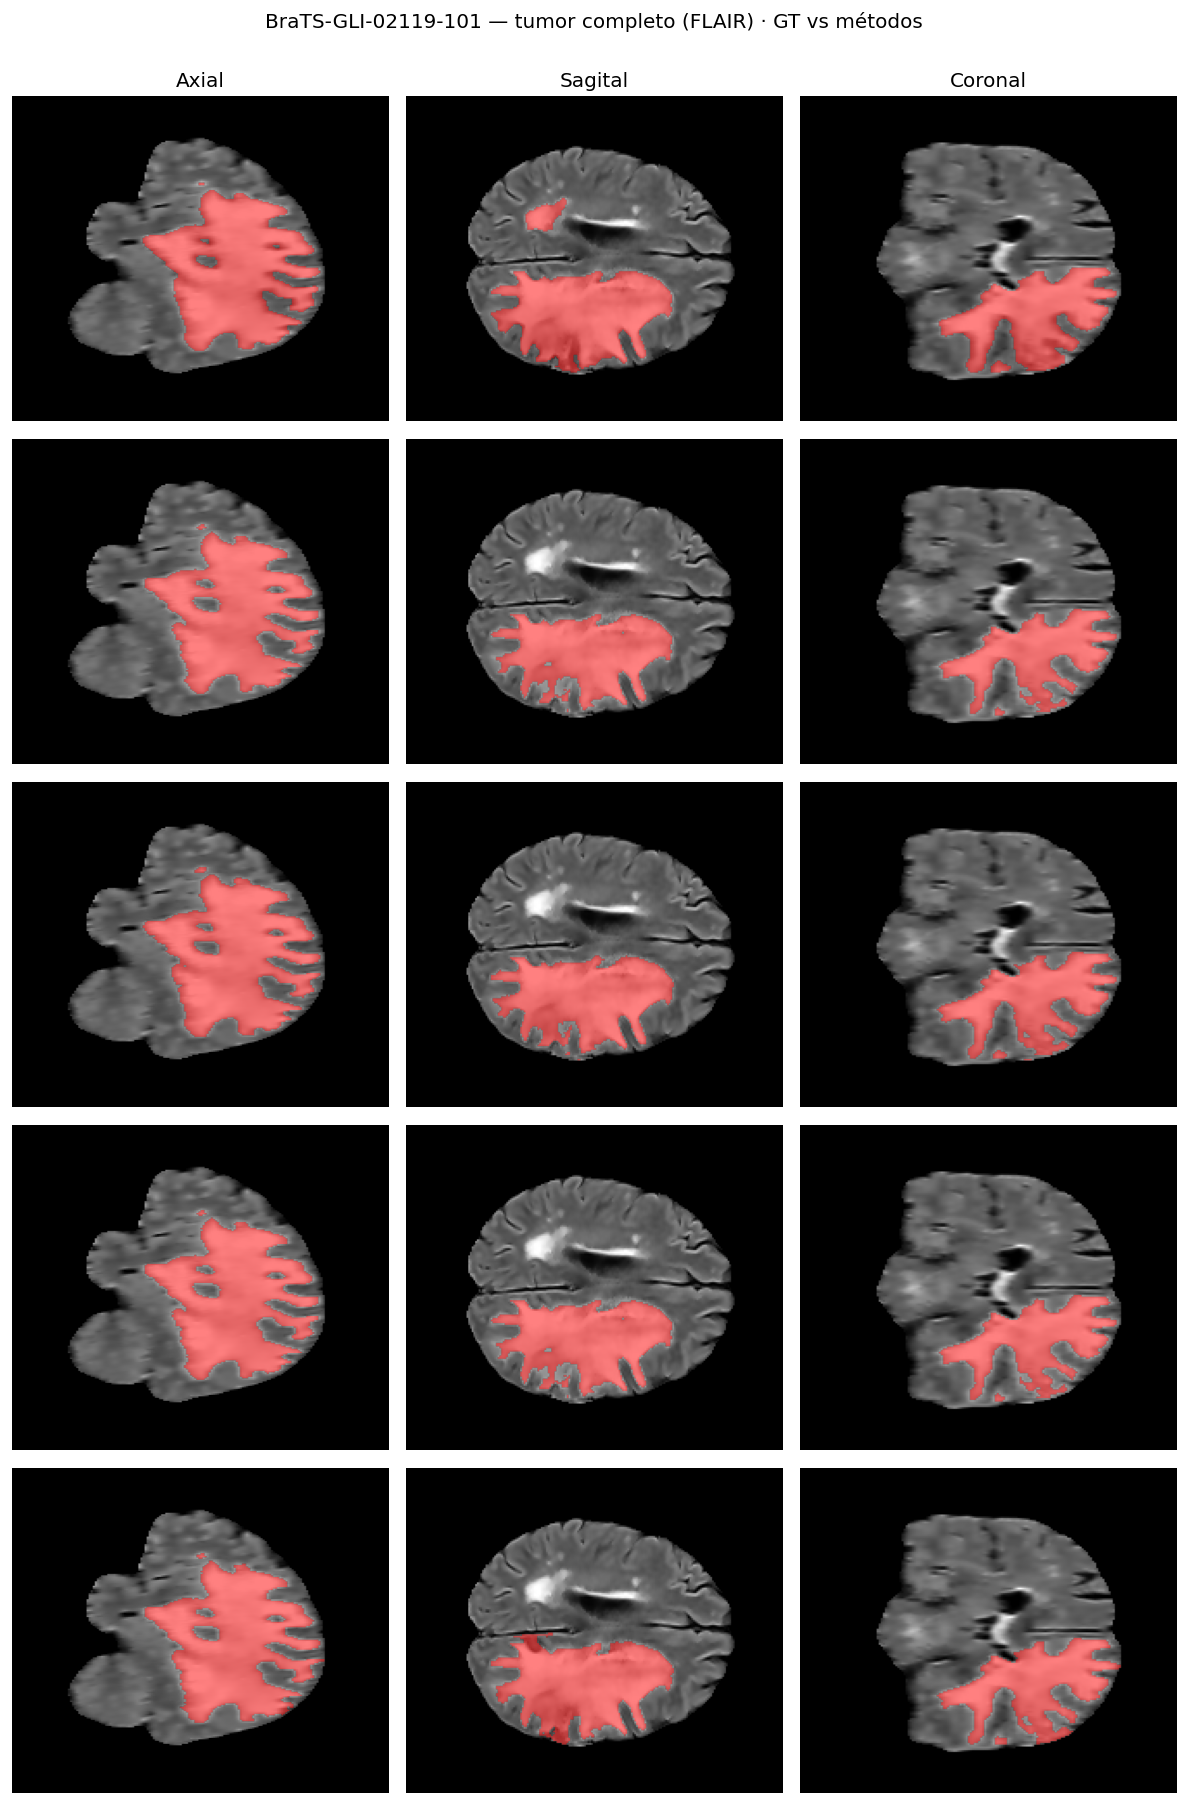
\includegraphics[width=\columnwidth]{figuras/seg_comparacion_02119-101.png}
\caption{Caso BraTS-GLI-02119-101 (tumor grande): comparativa
GT vs.\ Otsu, GMM, crecimiento de regiones y watershed sobre el
volumen FLAIR preprocesado. Es el único caso donde los cuatro
métodos producen Dice$>0{,}89$.}
\label{fig:seg_02119}
\end{figure}

\begin{figure}[H]
\centering
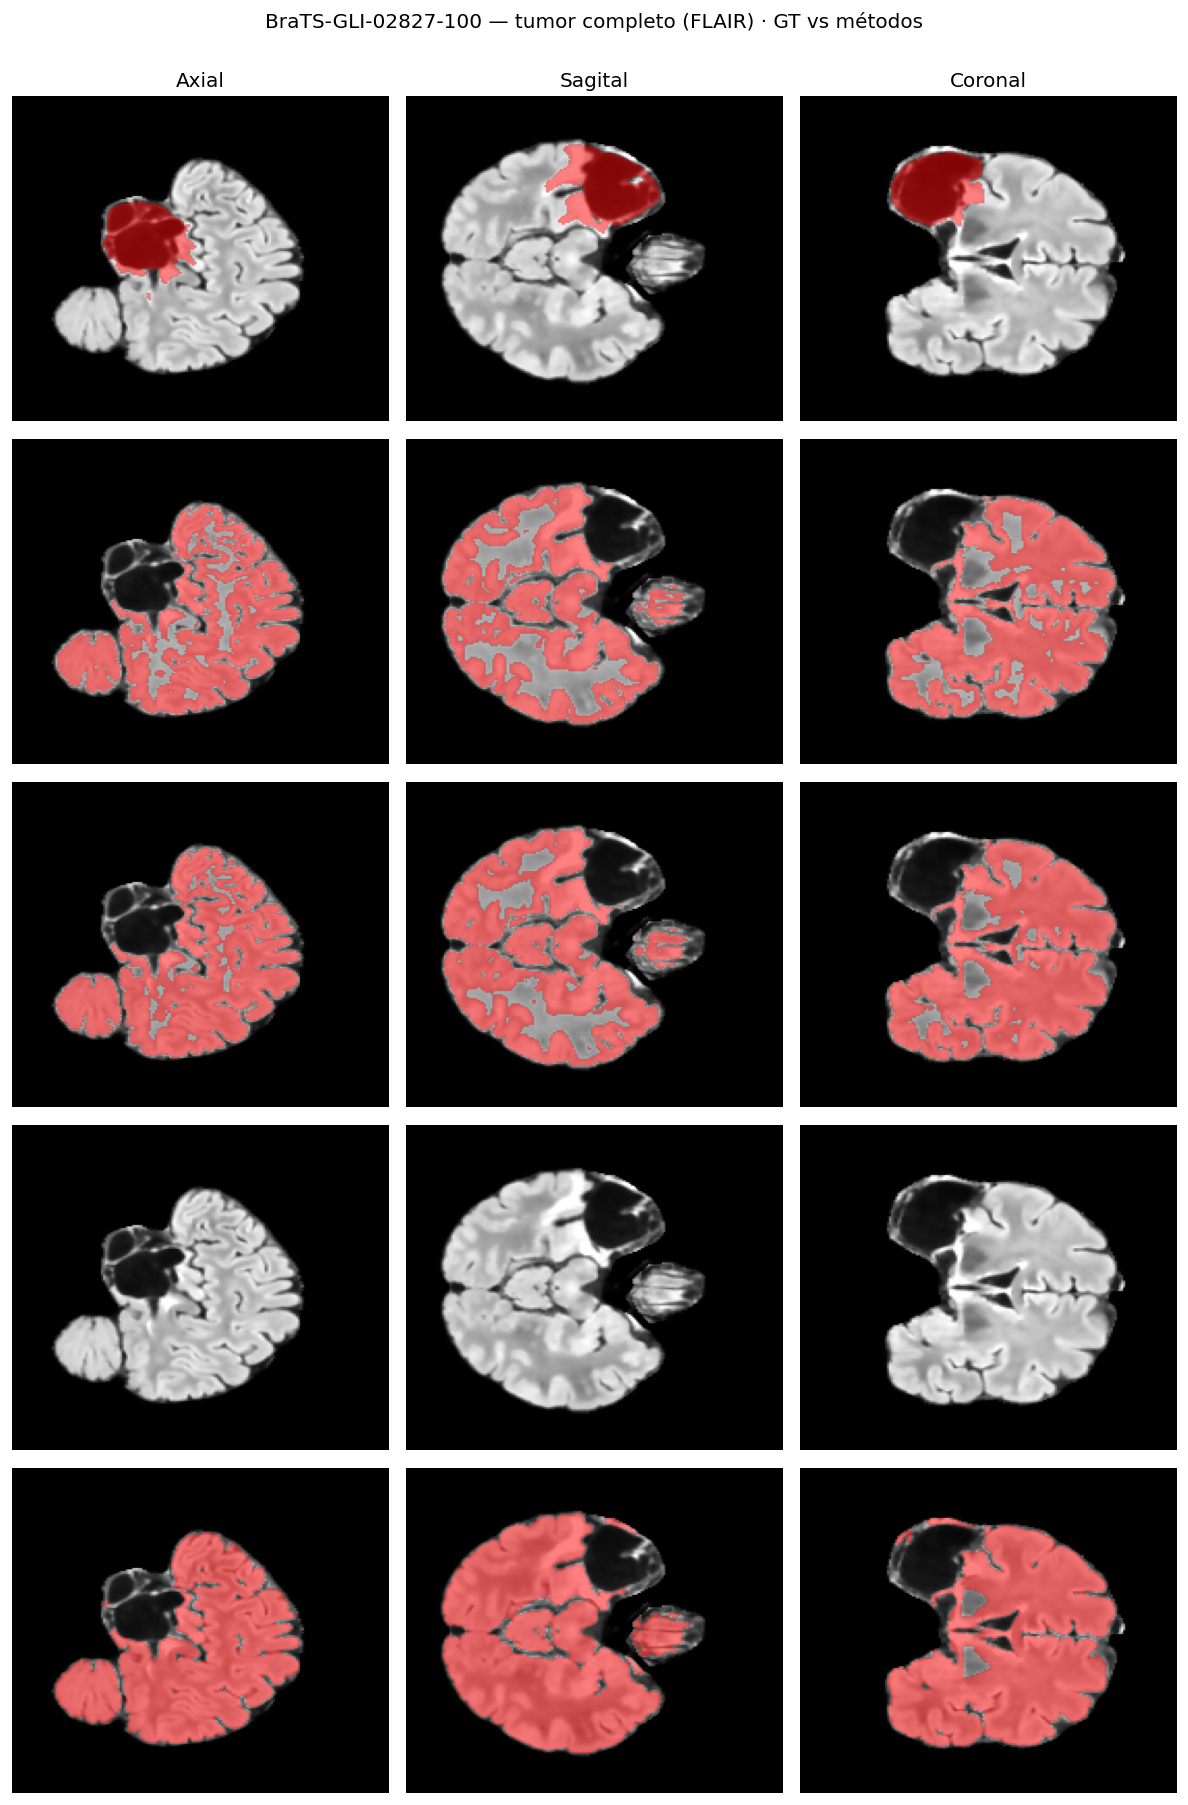
\includegraphics[width=\columnwidth]{figuras/seg_comparacion_02827-100.png}
\caption{Caso BraTS-GLI-02827-100 (típico, dominado por cavidad
de resección): la hipointensidad de la RC en FLAIR rompe la
hipótesis de un único modo brillante y todos los métodos
fracasan.}
\label{fig:seg_02827}
\end{figure}

\begin{figure}[H]
\centering
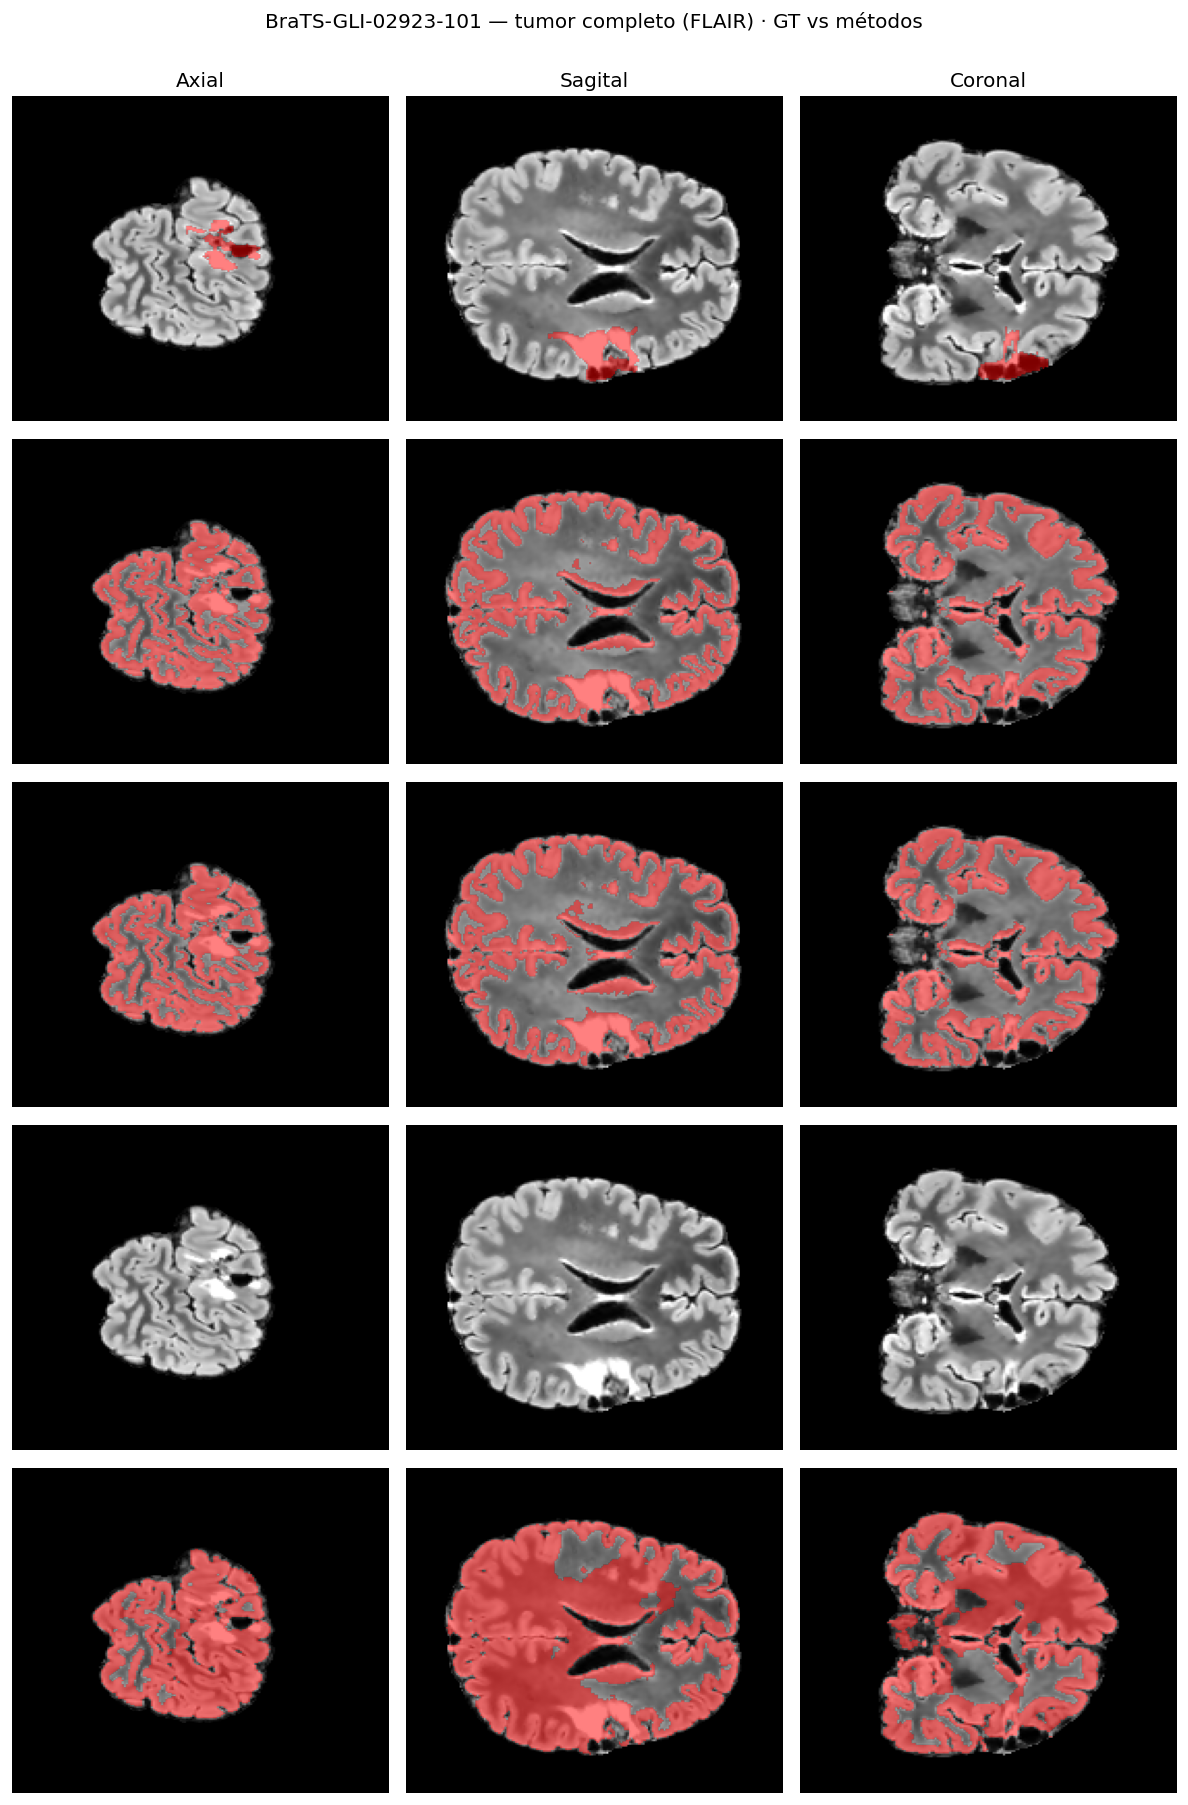
\includegraphics[width=\columnwidth]{figuras/seg_comparacion_02923-101.png}
\caption{Caso BraTS-GLI-02923-101 (tumor pequeño): la fracción
tumor/encéfalo es tan baja que los métodos globales saturan en
falsos positivos y el crecimiento sembrado en el centroide del
GT no logra propagarse.}
\label{fig:seg_02923}
\end{figure}

% =====================================================================
\section{Registro rígido demostrativo}
\label{sec:reg}
% =====================================================================
El bloque de registro implementa un motor clásico de
alineamiento volumen-volumen basado en
\textbf{Información Mutua de Mattes} con una transformación
\textbf{rígida Euler3D} (3 rotaciones + 3 traslaciones,
6\,d.o.f.) y un esquema piramidal multi-resolución, todo sobre
SimpleITK. Como el EDA estableció que las modalidades de BraTS
ya están coregistradas, el experimento es \textbf{demostrativo}:
se toma el volumen T1n original como \emph{moving},
se le aplica una transformación rígida conocida y se mide la
capacidad del motor para recuperarla.

\subsection{Configuración}
Los hiperparámetros se cargaron desde
\texttt{parametros\_usados.json} y se resumen en la
Tabla~\ref{tab:reg_param}.

\begin{table}[H]
\centering
\caption{Parámetros del registro Mattes\,MI + Euler3D
multi-resolución.}
\label{tab:reg_param}
\small
\begin{tabular}{ll}
\toprule
Parámetro & Valor \\
\midrule
Modalidad fija/móvil       & T1n \\
Métrica                    & Mattes Mutual Information \\
Bins del histograma (MI)   & 50 \\
Fracción de muestreo       & 0.1 (seed=42) \\
Iteraciones máx.\ por nivel& 150 \\
Pirámide --- \emph{shrink} & $[4,\,2]$ \\
Pirámide --- $\sigma$      & $[2,\,1]$ \\
Optimizador                & Gradient Descent Line Search \\
Inicialización             & \texttt{CenteredTransformInitializer} (geom.) \\
Rotación perturbada (°)    & $(6{,}0,\,4{,}0,\,-5{,}0)$ \\
Traslación perturbada (mm) & $(5{,}0,\,-4{,}0,\,3{,}0)$ \\
\bottomrule
\end{tabular}
\end{table}

\subsection{Métricas por caso}
La Tabla~\ref{tab:reg_metricas} reporta las métricas de los tres
casos registrados. \textbf{TRE} (\emph{Target Registration Error})
se calcula sobre puntos de control distribuidos en el volumen y
es la métrica más fiable; \textbf{Dice de cerebro} se calcula
entre las máscaras del encéfalo de fijo y móvil antes/después
del registro; \textbf{MSE} es el error cuadrático medio de
intensidades; \textbf{MI final} es el valor de la métrica de
Mattes al converger (más negativo = mejor).

\begin{table}[H]
\centering
\caption{Métricas de registro por caso (3 casos). Sub-vóxel en
todos los TRE.}
\label{tab:reg_metricas}
\small
\setlength{\tabcolsep}{3pt}
\resizebox{\columnwidth}{!}{%
\begin{tabular}{lccccccc}
\toprule
Caso & \makecell{TRE\\(mm)} & \makecell{Dice\\antes} & \makecell{Dice\\desp.} & \makecell{MSE\\antes} & \makecell{MSE\\desp.} & \makecell{MI\\final} & \makecell{Tiempo\\(s)} \\
\midrule
02827-100 & \cellcolor{cellgood}0.0021 & 0.907 & \cellcolor{cellgood}0.963 & 15731.86  & 110.81   & -1.196 & 107.0 \\
02119-101 & \cellcolor{cellgood}0.0029 & 0.913 & \cellcolor{cellgood}0.963 & 1793.01   & 35.69    & -1.141 & 90.5 \\
02923-101 & \cellcolor{cellgood}0.0058 & 0.915 & \cellcolor{cellgood}0.965 & 215758.45 & 4325.13  & -1.263 & 88.7 \\
\midrule
\textbf{Promedio} & \cellcolor{cellgood}\textbf{0.0036} & \textbf{0.912} & \cellcolor{cellgood}\textbf{0.964} & --- & --- & \textbf{-1.200} & \textbf{95.4} \\
\bottomrule
\end{tabular}}
\end{table}

\subsection{Visualización}
Las Figuras~\ref{fig:reg_02119}--\ref{fig:reg_02923} muestran,
para cada caso, los tres volúmenes ---fijo (referencia), móvil
desalineado y móvil recuperado--- en una vista axial central.
La Figura~\ref{fig:reg_conv} muestra las curvas de convergencia
de la métrica Mattes por iteración y por nivel piramidal en los
tres casos.

\begin{figure}[H]
\centering
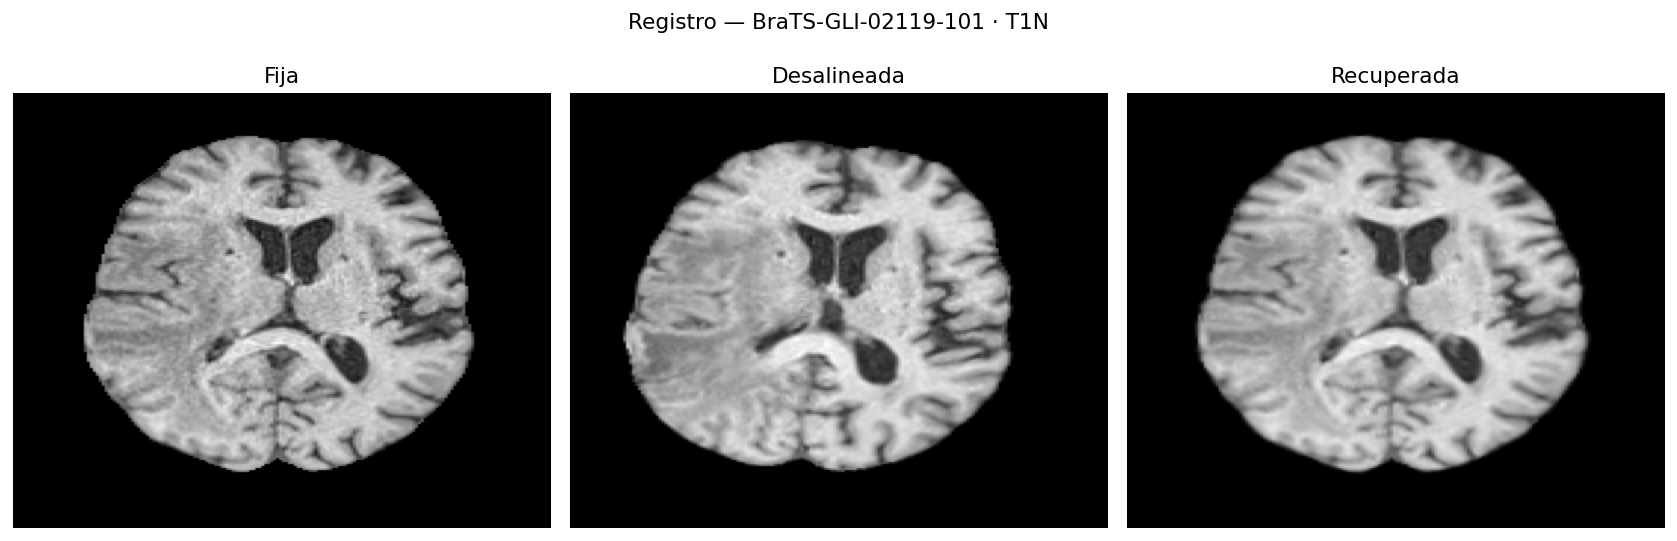
\includegraphics[width=\columnwidth]{figuras/reg_02119-101.png}
\caption{Caso BraTS-GLI-02119-101: \emph{fijo} (izq.),
\emph{desalineado} (centro) y \emph{recuperado} (der.) tras el
registro rígido. TRE residual $=0{,}0029$\,mm.}
\label{fig:reg_02119}
\end{figure}

\begin{figure}[H]
\centering
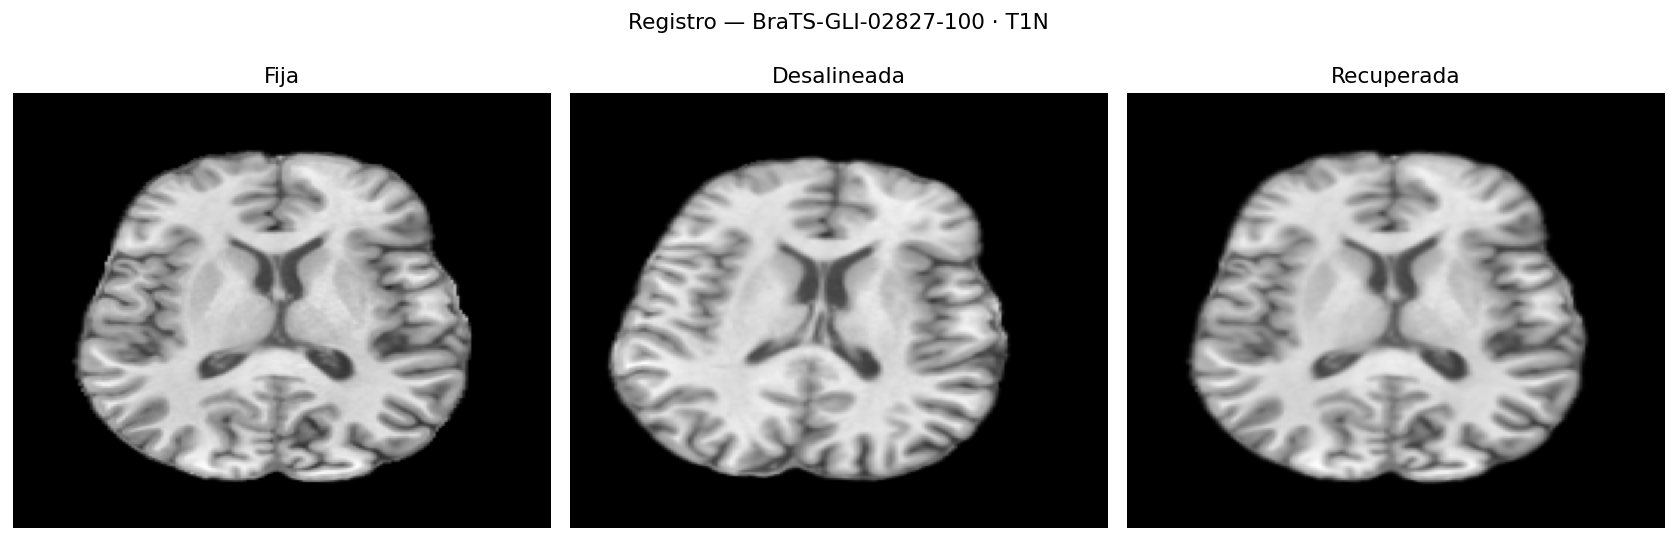
\includegraphics[width=\columnwidth]{figuras/reg_02827-100.png}
\caption{Caso BraTS-GLI-02827-100: TRE residual
$=0{,}0021$\,mm, el mejor de los tres.}
\label{fig:reg_02827}
\end{figure}

\begin{figure}[H]
\centering
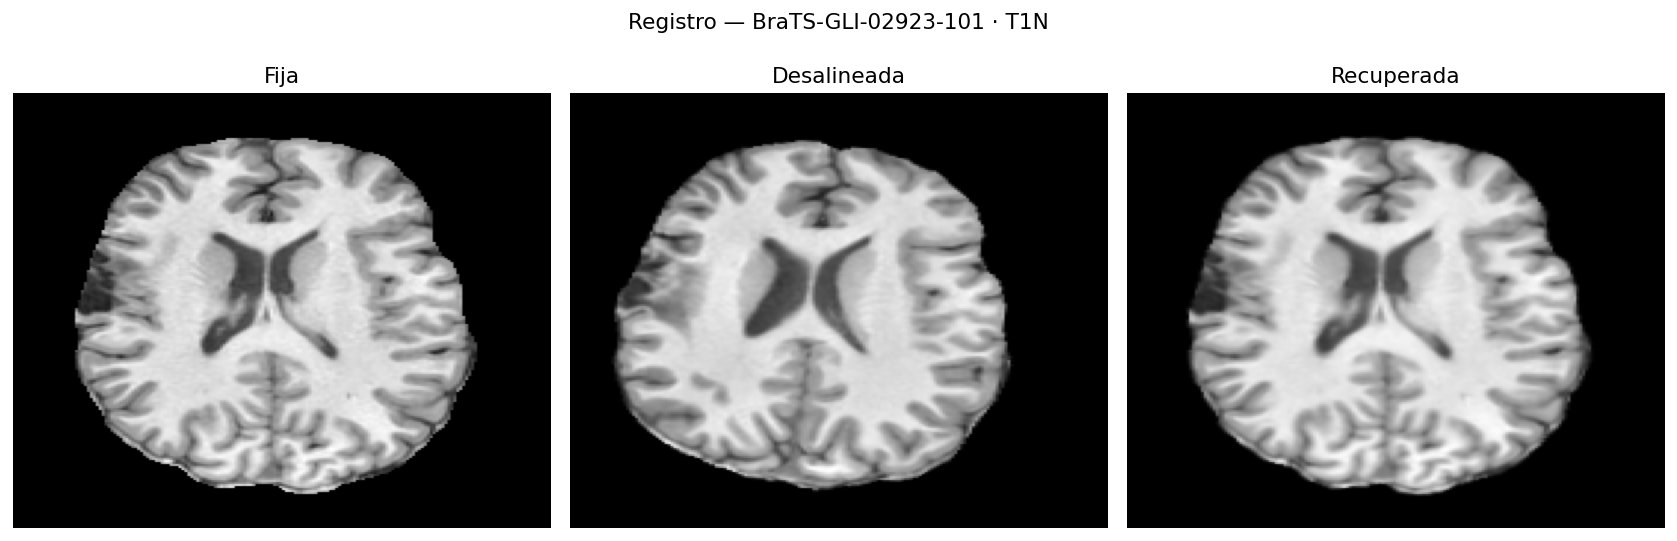
\includegraphics[width=\columnwidth]{figuras/reg_02923-101.png}
\caption{Caso BraTS-GLI-02923-101: TRE residual
$=0{,}0058$\,mm, todavía sub-vóxel.}
\label{fig:reg_02923}
\end{figure}

\begin{figure}[H]
\centering
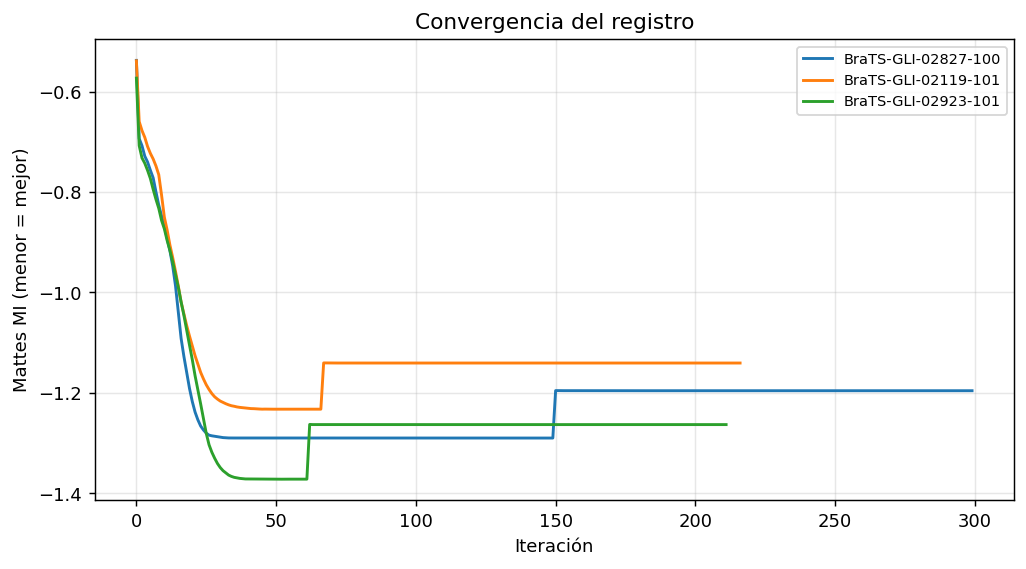
\includegraphics[width=\columnwidth]{figuras/reg_convergencia.png}
\caption{Curvas de convergencia de la métrica de Mattes (negativa
de la información mutua) por iteración y por nivel piramidal,
para los tres casos.}
\label{fig:reg_conv}
\end{figure}

% =====================================================================
\section{Discusión y limitaciones}
\label{sec:disc}
% =====================================================================
\subsection{Por qué fallan los métodos clásicos en el tumor
completo}
La Tabla~\ref{tab:seg_detalle} expone un patrón inequívoco: los
cuatro métodos basados únicamente en intensidad sólo rinden bien
en el caso 02119-101, donde la sub-región dominante es la SNFH
($\sim 174\,$k vóxeles, hiperintensa en FLAIR). En los otros
cuatro casos hay siempre un componente sustancial de RC ---por
ejemplo $43{,}8\,$k vóxeles de RC frente a $13{,}2\,$k de SNFH
en 02827-100, o $88{,}8\,$k frente a $62{,}3\,$k en 02514-102---
y la RC es \textbf{hipointensa} en FLAIR, indistinguible del
ventrículo o del líquido cefalorraquídeo.

En consecuencia, el objetivo \texttt{seg > 0} contiene
simultáneamente vóxeles brillantes (SNFH/ET) y vóxeles oscuros
(RC) que no pueden separarse con un único umbral global ---ni con
una mezcla Gaussiana de pocos componentes que asigne la RC a la
misma clase que SNFH---. El crecimiento de regiones, sembrado en
el centroide del GT, queda atrapado en una sola sub-región: si
la semilla cae en RC, no propaga a SNFH y viceversa. La
sensibilidad media de $0{,}163$ de este método refleja esta
fragmentación.

El watershed obtiene la mayor sensibilidad media ($0{,}638$) pero
su precisión es la peor a igualdad de Dice, evidenciando
sobre-segmentación. La conclusión práctica es robusta:
\textbf{los métodos clásicos basados en intensidad son
insuficientes para segmentar el tumor completo post-tratamiento}
en BraTS 2024 GLI. Resolver este problema requiere o bien
información de forma (atlas, modelos estadísticos),
multi-modalidad explícita (combinar FLAIR + T1c) o aprendizaje
supervisado, ninguna de las cuales pertenece al alcance del
presente proyecto.

\subsection{Limitaciones del registro demostrativo}
El registro alcanza un TRE residual sub-vóxel ($\leq 0{,}006$\,mm)
en los tres casos y eleva el Dice de cerebro de $0{,}91$ a
$0{,}96$, lo que confirma la corrección del motor. No obstante,
caben dos matices:

\begin{enumerate}
  \item La validación es \emph{intra-sujeto} y \emph{sintética}:
        la transformación recuperada es la misma que se aplicó
        artificialmente, lo que sobreestima el desempeño frente a
        un escenario clínico real con diferencias inter-sujeto.
  \item La transformación es \emph{rígida} y no compensa
        deformaciones locales (desplazamiento de masa, atrofia,
        cavidad de resección). Para esos escenarios se requeriría
        un registro deformable (B-spline, Demons, SyN).
\end{enumerate}

% =====================================================================
\section{Reproducibilidad}
\label{sec:repro}
% =====================================================================
\begin{itemize}
  \item \textbf{Modalidad de segmentación:} T2-FLAIR (\texttt{t2f}).
  \item \textbf{Objetivo:} tumor completo (\texttt{seg > 0}).
  \item \textbf{Pipeline de limpieza:} Wiener (size=3) $\to$ N4
        (shrink=4) $\to$ normalización por percentiles
        $(p_{0{,}5},\,p_{99{,}5})$.
  \item \textbf{Métodos clásicos:} Otsu multinivel (2 cortes),
        GMM (3 componentes), \texttt{ConnectedThreshold} (semilla
        en el centroide del GT), watershed por marcadores sobre
        magnitud del gradiente.
  \item \textbf{Modalidad de registro:} T1n.
  \item \textbf{Métrica/transformación:} Mattes\,MI (50 bins,
        muestreo $0{,}1$) + Euler3D, multi-resolución
        shrink $[4,2]$ / $\sigma\,[2,1]$, máximo 150 iteraciones
        por nivel, inicialización \texttt{CenteredTransform\-Initializer}
        (geometría).
  \item \textbf{Perturbación:} rotación $(6{,}4{,}-5)^{\circ}$ y
        traslación $(5,-4,3)$\,mm.
  \item \textbf{Casos demostrativos:} 02119-101, 02827-100,
        02923-101, 02514-102, 02859-100 (segmentación) y
        02119-101, 02827-100, 02923-101 (registro).
  \item \textbf{Código y artefactos:}
        \url{https://github.com/AbelAlbuez/medical-image-processing}.
\end{itemize}

% =====================================================================
\section{Conclusiones y trabajo futuro}
\label{sec:conclu}
% =====================================================================
El proyecto cubre las tres tareas requeridas
---EDA, segmentación y registro--- sobre BraTS 2024 GLI sin
recurrir a aprendizaje profundo. El EDA cuantitativo justifica la
elección de FLAIR para segmentar el tumor completo (mayor
separabilidad de SNFH frente a tejido sano) y fija parámetros
operativos para el registro. La segmentación clásica obtiene
resultados aceptables \textbf{únicamente cuando la sub-región
dominante es la SNFH hiperintensa}; en presencia de cavidad de
resección o tumor pequeño, todos los métodos colapsan, con un
Dice agregado máximo de $0{,}33$ (Otsu). Este resultado es el
hallazgo central del proyecto y constituye una motivación
empírica clara para el uso de métodos basados en aprendizaje en
contextos clínicos reales. El bloque de registro, en cambio,
recupera con precisión sub-vóxel una perturbación rígida conocida
en los tres casos, validando la implementación del motor
Mattes\,MI\,+\,Euler3D multi-resolución.

\textbf{Trabajo futuro:} (i) extender la segmentación a estrategias
multi-modalidad (combinaciones FLAIR\,+\,T1c) y a operadores
morfológicos para imponer compacidad; (ii) reemplazar el
crecimiento de regiones por un \emph{level-set} con término de
forma; (iii) probar un registro deformable (Demons o B-spline)
para los casos con masa significativa; y (iv) ampliar la cohorte
de evaluación a la totalidad del subset GLI.

% =====================================================================
% Bibliografía
% =====================================================================
\begin{thebibliography}{9}

\bibitem{baid2021brats}
U.~Baid \emph{et al.},
``The RSNA-ASNR-MICCAI BraTS 2021 benchmark on brain tumor
segmentation and radiogenomic classification,''
\emph{arXiv:2107.02314}, 2021.

\bibitem{lloyd2010itk}
B.~C.~Lowekamp, D.~T.~Chen, L.~Ibáñez and D.~Blezek,
``The design of SimpleITK,''
\emph{Frontiers in Neuroinformatics}, vol.~7, p.~45, 2013.

\bibitem{otsu1979}
N.~Otsu,
``A threshold selection method from gray-level histograms,''
\emph{IEEE Trans.\ Syst., Man, Cybern.}, vol.~9, no.~1,
pp.~62--66, 1979.

\bibitem{tustison2010n4}
N.~J.~Tustison \emph{et al.},
``N4ITK: Improved N3 bias correction,''
\emph{IEEE Trans.\ Med.\ Imag.}, vol.~29, no.~6,
pp.~1310--1320, 2010.

\bibitem{mattes2003}
D.~Mattes, D.~R.~Haynor, H.~Vesselle, T.~K.~Lewellyn
and W.~Eubank,
``PET-CT image registration in the chest using free-form
deformations,''
\emph{IEEE Trans.\ Med.\ Imag.}, vol.~22, no.~1, pp.~120--128,
2003.

\bibitem{vincent1991watersheds}
L.~Vincent and P.~Soille,
``Watersheds in digital spaces: an efficient algorithm based on
immersion simulations,''
\emph{IEEE Trans.\ Pattern Anal.\ Mach.\ Intell.}, vol.~13,
no.~6, pp.~583--598, 1991.

\end{thebibliography}

\end{document}
